./\newcommand{\code}[1]{\texttt{#1}}

\section{Non-conjunctive Partial Deduction}

\begin{figure}[!t]
  \centering
  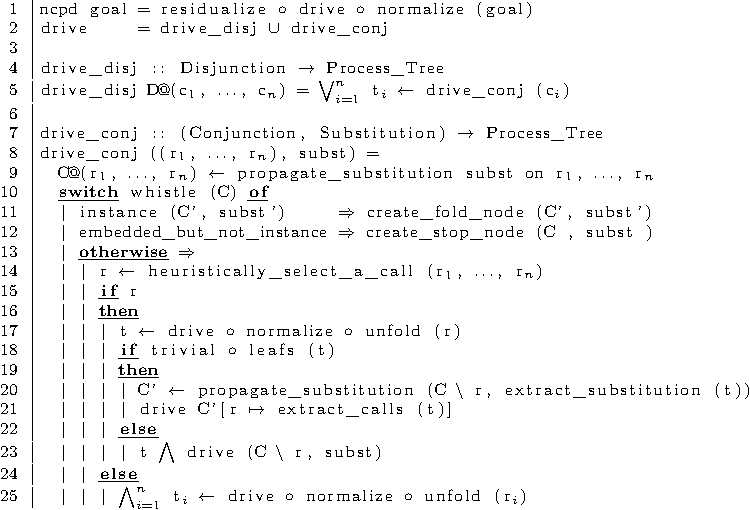
\includegraphics[width=0.85\textwidth]{algo_pseudo-crop.pdf}
  \caption{\db{Non-conjunctive Partial Deduction Pseudo Code}}
  \label{fig:ncpd-pseudo}
\end{figure}

In this section we describe a novel approach to specialization of relational programs.
This approach draws inspiration from both conjunctive partial deduction and supercompilation.
The aim was to create a specialization algorithm which is simpler than conjunctive partial deduction and uses properties of \mk{} to improve performance of the input programs.

The algorithm pseudocode is shown on Fig.~\ref{fig:ncpd-pseudo}.
For the sake of brevity and clarity, we provide functions \code{drive\_disj} and \code{drive\_conj} which describe how to process disjunctions and conjunctions respectively.
Driving itself is a trivial combination of presented functions (line 2).

A driving process creates a process tree, from which a residual program is later created.
The process tree is meant to mimic the execution of the input program.
The nodes of process tree include a \emph{configuraion} which describes the state of program evaluation at some point.
In our case configuration is a conjunction of relation calls.
The substitution computed at each step is also stored in the tree node, although it is not included into the configuration.

Hereafter, we consider all goals and relation bodies to be in \emph{canonical normal form}~---~a disjunction of conjunctions of either calls or unifications.
Moreover, we assume all fresh variables to be introduced into scope and all unifications to be computed at each step.
Those disjuncts in which unifications fail are removed.
Other disjuncts take form of a conjunction of relation calls accompanied with a substitution computed from unificaitons.
Any miniKanren term can be trivially transformed to the described form.
In Fig.~\ref{fig:ncpd-pseudo} function \code{normalize} is assumed to perform term normalization.
The code is omitted for brevity.


% The very first step of driving a conjunction is to apply a substitution to the variables in relation calls (line 10).

There are several core ideas behind this algorithm.
The first is to select an arbitrary relation to unfold, not necessarily the leftmost which is safe.
The second idea is to use a heuristic which decides if unfolding a relation call can lead to discovery of contradictions between conjuncts which in turn leads to restriction of the answer set at specialization-time \db{(line 14; \code{heuristically\_select\_a\_call} stands for heurictics combination, the exact code is omitted)}.
If those contradictions are found, then they are exposed by considering the conjunction as a whole and substituting the result of the call unfolding back into the conjunction the call was selected from thus \emph{joining} the conjunction back together instead of using \emph{split} as in CPD \db{(lines 15--23)}.
Finally, if the heuristic fails to select a potentially good call, then the conjunction is splitted into individual calls which are driven in isolation and are never joined \db{(line 25)}.

When the heuristic selects a call to unfold (lines 14--15), a process tree is constructed for the selected call \emph{in isolation} (line 17).
The leaves of the computed tree are examined.
If all leaves are either computed substitutions or are renamings of some relations accompanied with non-empty substitutions, then the leaves are collected and replace the considered call in the root conjunction (lines \db{20--21}).
If the selected call does not suit the criteria, the results of its unfolding is not propagated onto other relation calls withing the conjunction and the next suitable call is selected (line \db{23}).
According to the denotational semantics of \mk{} it is safe to compute individual conjuncts in any order, thus it is ok to drive any call and then propagate its results onto the other calls.

% Each time we examine a conjunction of calls, we \emph{split} them into separate nodes which are driven independently from each other.
% Among the relation calls we select one which is according to the heuristic is likely to narrow down the answer set \db{(line 15)}.
% If the selected call does not suit the criteria, the results of its unfolding is not propagated onto other relation calls withing the conjunction and the next suitable call is selected \db{(line 22)}.

This process creates branchings whenever a disjunction is examined lines 4--\db{5}).
At each step we make sure that we do not start driving a conjunction which we have already examined.
To do this, we check if the current conjunction is renaming of any other configuration in the tree (line \db{11}).
If it is, then we create a special node which then is residualized into a call to the corresponding relation.
This is known as \emph{folding} in supercompilation.

We decided not to perform generalization in this approach in the same fashion as CPD or supercompilation does.
Our conjunctions are always splitted into individual calls and are joined back together if it is sensible.
If the need for generalization arises, i.e. embedding is detected, then we immediately stop driving this conjunction (line \db{12}).
When redisualizatin such conjunction, we just generate a conjunction of calls to the input program before specialization.

% The generalization is used in supercompilation and partial deduction to ensure termination at the same time as some degree of specialization.
% The generalization of two terms is usually a \emph{most-specific generalization}.
% Generalization is used to abstract away some information computed during driving.
% In conjunctive partial deduction generalization is modified to support treating of conjunctions.
% The generalization selects subconjuctions of two conjuncts which are similar (call to the same relation and their arguments have similar shape and distribution).
% For the subconjunctions selected a most-specific generalization is computed.

% In our approach we only do splitting of a conjunction into individual relation calls.
% This makes any program with an accumulating parameter to be a problem.
% Sometimes when there is a need to do a proper generalization, it is in reality just an instance of some other goal within the tree and we can simply create a call there \db{(line 13)}.
% Otherwise we are unable to meaningfully specialize such goal, but we can always just include the initial program in the residual program and call the corresponding relation.


\subsection{Unfolding}

Unfolding in our case is done by substitution of some relation call by its body with simultaneous normalization and computation of unifications.
% To unfold a relation call we do the following steps.
% \db{TODO: the following has alredy mentioned above.}
% First, the formal arguments of a relation are substituted for the actual arguments of the call in the body.
% All fresh variables get instantiated.
% The body is transformed into a canonical form (disjunction of conjunctions of either calls or unifications).
% All unifications are computed.
% Those disjuncts in which unifications fails are removed.
% Other disjuncts take form of a conjunction of relation calls accompanied with a substitution.
The unfolding itself is straightforward however it is not always clear what to unfold and when to \emph{stop} unfolding.
Unfolding in functional programming languages specialization, as well as inlining in imperative one, is usually considered to be safe from a residual program efficiency point of view.
It may only lead to code explosion or code duplication which is mostly left to a target program compiler optimization or even is out of consideration at all if a specializer is considered as a standalone tool~\cite{jonesbook}.

Unfortunately, this is not the case for the specialization of relational programming language.
Unlike functional and imperative, in logic and relational programming language unfolding may easily affect the target program efficiency~\cite{leuschel2002logic}.
Unfolding too much may create extra unifications, which is by itself a costly operation, or even introduce duplicated computations by propagating the unfolding results onto neighboring conjuncts.

There is a fine edge between too much unfolding and not enough unfolding.
The former may be even worse than the latter.
We believe that the following heuristic provides a reasonable approach to controling unfolding.

\subsection{Heuristic}

The intuition behind the heuristic is to find those calls which are safe to unfold.
We deem every static conjunct (non-recursive) to be safe because they never lead to growth in the number of conjunctions.
Those calls which unfold deterministically, meaning there is only one disjunct in the unfolded relation, are also considered to be safe.

The other more complicated case is when there are less disjuncts than there can possibly be.
This signifies that at least one branch of computations is gotten rid of.

The final heuristic selects the first conjunct which suites either of the following cases.
First we unfold those conjuncts which are static.
Then --- deterministic.
Then those which are less branching.
The last to be unfolded are those calls, which unfold to a substitution with not conjunction.

\subsection{Residualization}

Residualization is quite straightforward.
A branching in the process tree becomes a disjunction.
A split node becomes a conjunction.
Computed substitution is residualized as a conjunction of unifications.
A renaming node is just a call to a relation.
Relations are created for configurations on which leaf nodes are renamed.

One other thing is that when some configuration is occurred within the tree which is an instance of a configuration for which a new relation is created, then we just create a call.
